\chapter{Results and discussion}
\section{Scenario 1: one user and one basestation}


\subsection{The influence of the fly height on $SAR_{10g}$}
\label{sub:senario1_influenceOfFlyHeight}

This section investigates how the fly height of the \gls{UABS} influence $SAR_{10g}$ and power consumption. In figure \ref{fig:fhsar}
becomes clear that with an increasing flyheight, the specific absorption rate grows exponentially which is also the case for the power consumption (fig. \ref{fig:pcsar})  

This behavior has been examined for the two types of antennae which are the fictional \gls{isotropicradiator} and the microstrip patch antenna. In figures 
\ref{fig:fhsar} and \ref{fig:pcsar} becomes clear that the type of antenna does not influence the power consumption nor the specific absorption rate in this  scenario.
The reasoning behind this is that the tool will possition the \gls{UABS} just above the user. An \gls{isotropicradiator} doesn't experience attenuation while a microstrip
patch antenna does. The later is however pointing to the ground meaning the user is in the perfect center of the main beam and therefore also
not experiencing any attenuation from the normalized radiation pattern.

\begin{figure}[th!]
  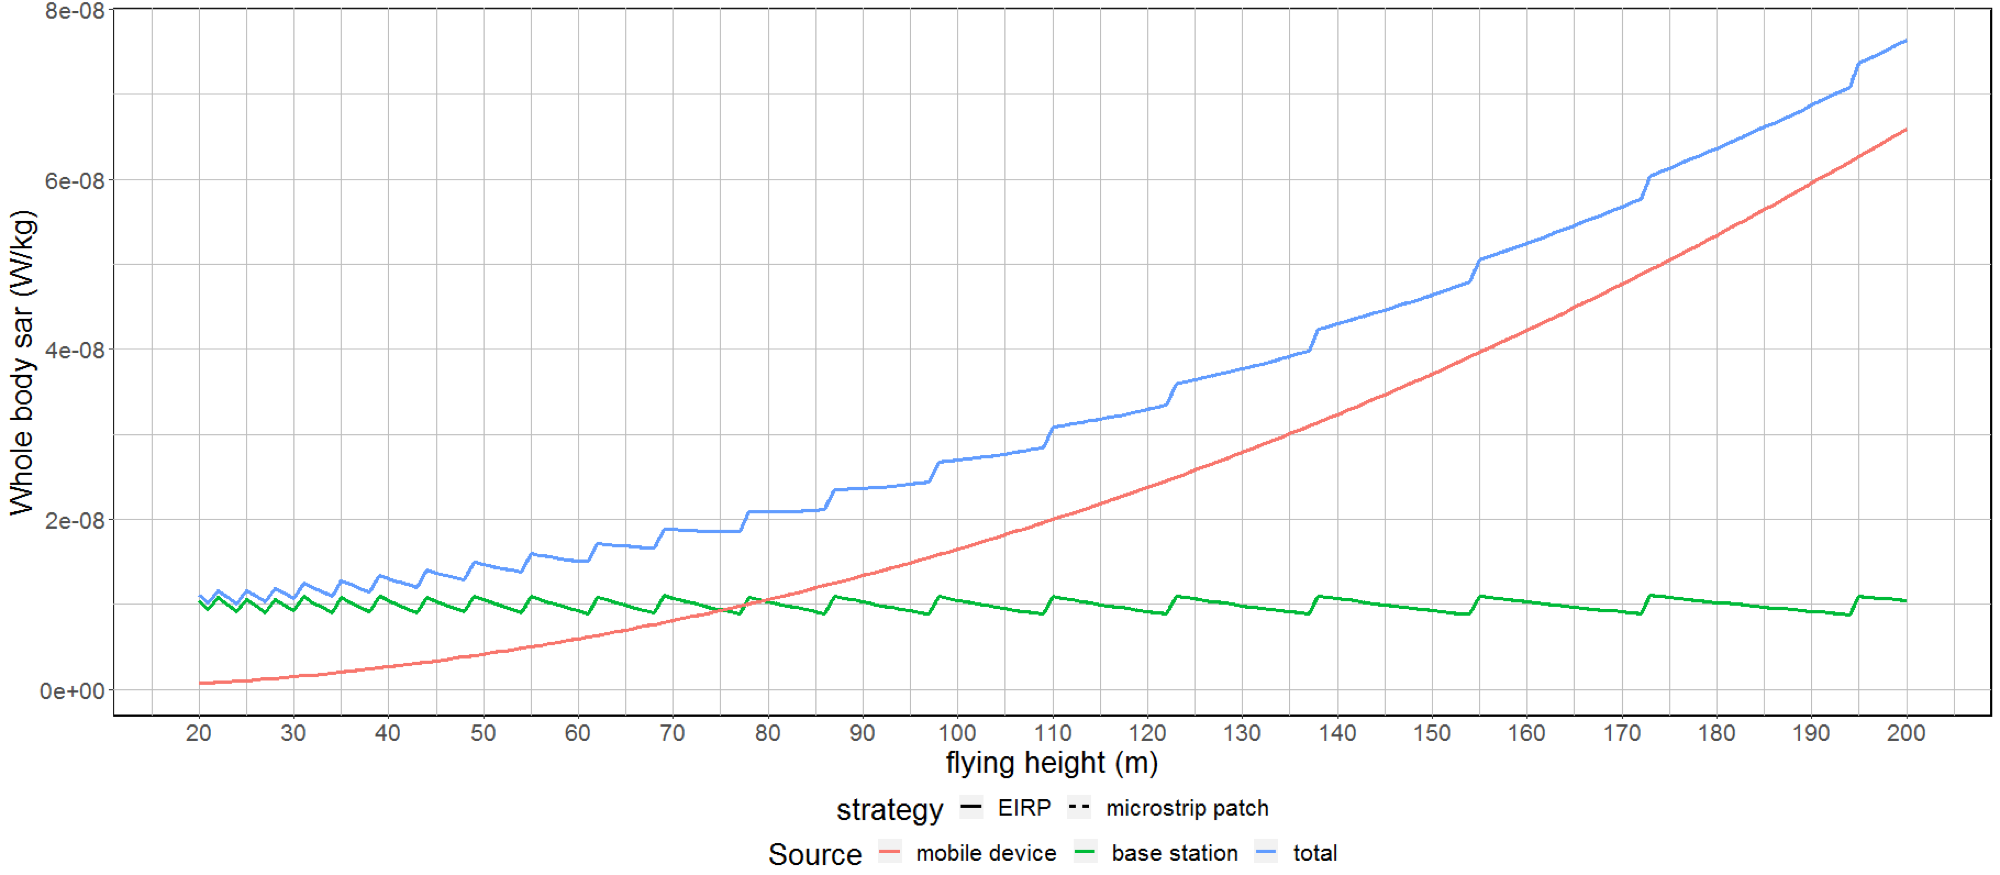
\includegraphics[width=\textwidth]{../results/s1/flyheight-sar.png}
  \caption{General design of a microstrip antenna}
  \label{fig:fhsar}
\end{figure}

\begin{figure}[bh!]
  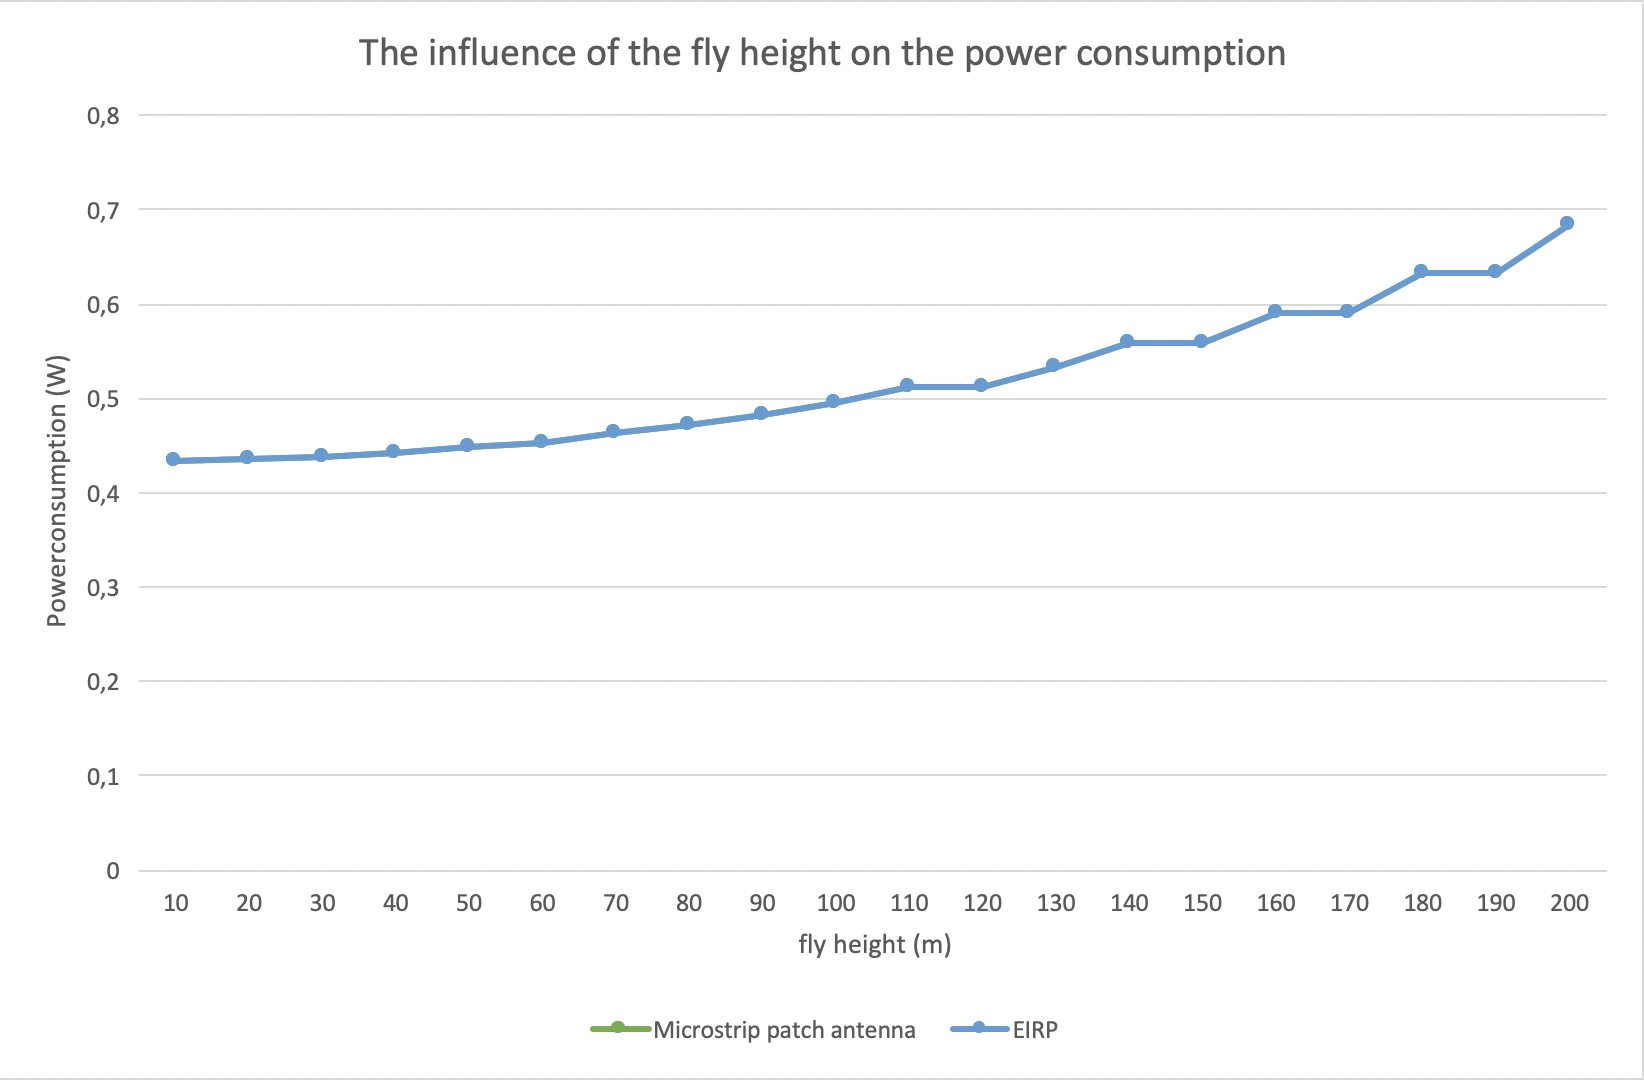
\includegraphics[width=\textwidth]{../results/s1/flyheight-pc.png}
  \caption{General design of a microstrip antenna}
  \label{fig:pcsar}
\end{figure}

\subsection{The influence from the maximum transmission power}
\gls{LTE} makes usages of power control meaning that no more power will be used then strictly necessary. The actual 
transmit power $P_{tx}$ therefore ranges between 0 and the maximum input power. $P_{tx}$ is zero when either no user is 
present or the user is so far away that the actual tranmit power would exceed the maximum transmission power.

Increasing the maximum tranmission power won't influence the power consumption or $SAR_{10g}$ because the \gls{UABS} won't use more
then strictly required. It is therefore more usefull to match the transmission power against a variable fly height. Figure \ref{fig:ptxfh}
shows a logarithmic  relationship showing that $P_{tx}$ increases fast at low altitude but slows down at lower altitudes. 

Since it became clear from section \ref{sub:senario1_influenceOfFlyHeight} that the type of antenna won't make a difference when applying
the tool in this scenario, it is not usefull to repeat this test with different types of antennae.


\begin{figure}[h!]
  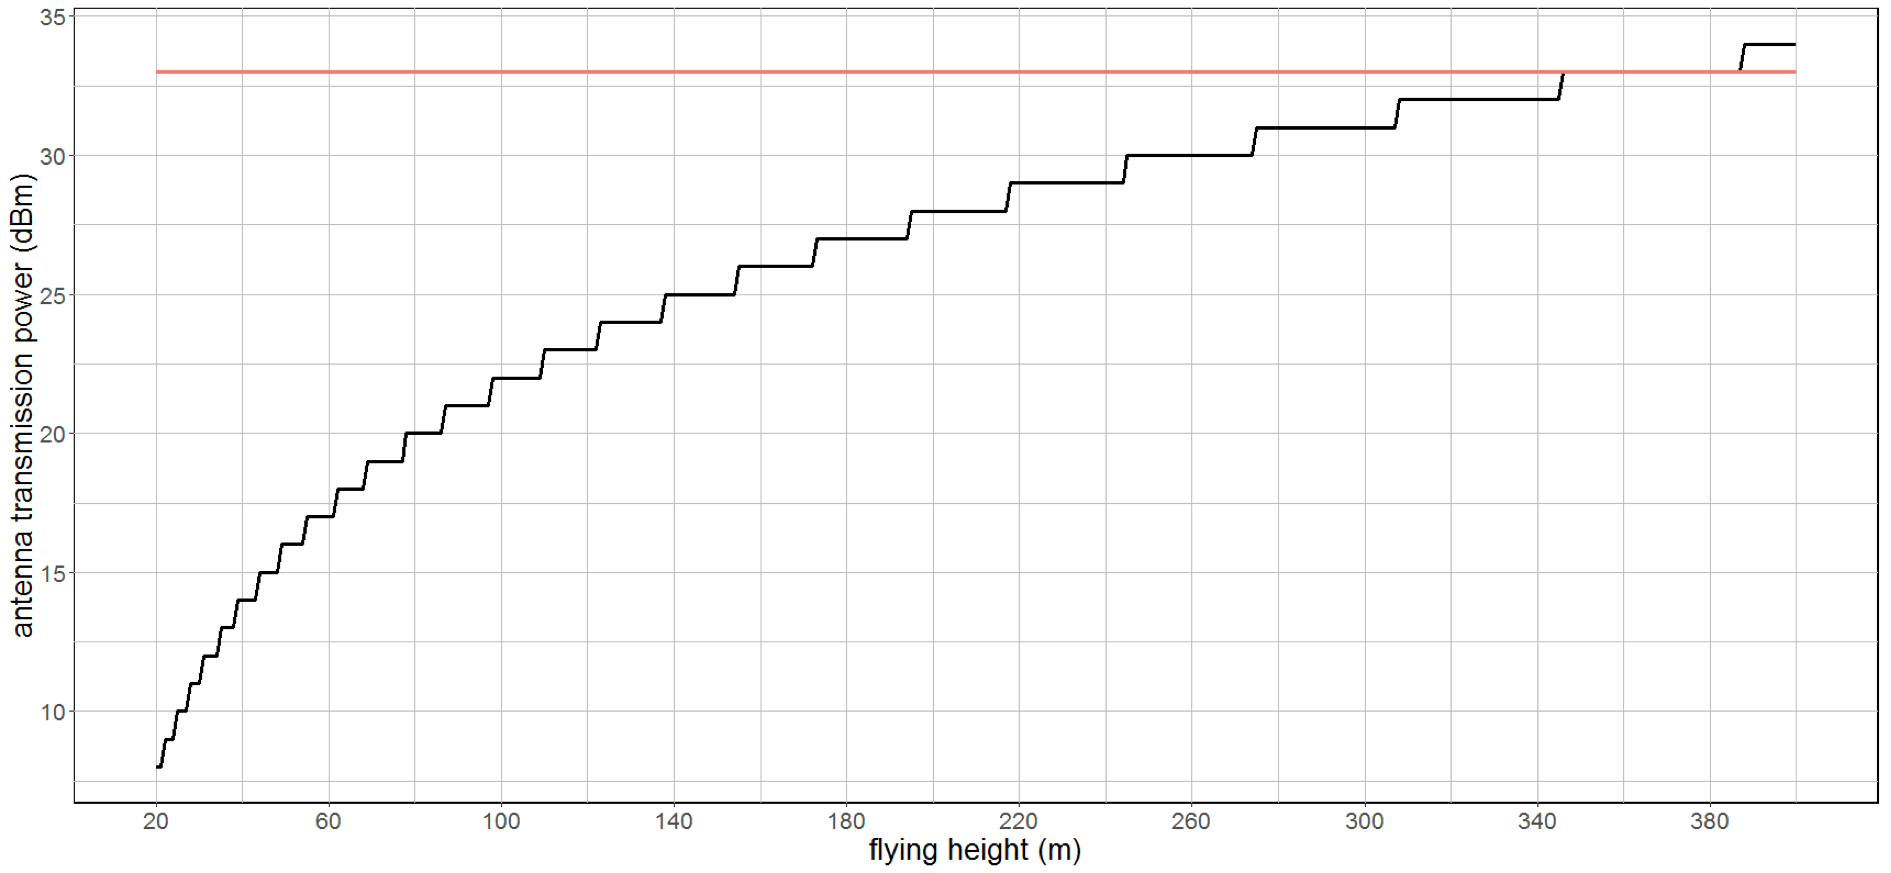
\includegraphics[width=\textwidth]{../results/s1/ptx-fh.png}
  \caption{General design of a microstrip antenna}
  \label{fig:ptxfh}
\end{figure}

\section{Scenario 2:}
\section{Scenario 3:}